\def\year{2015}
%File: formatting-instruction.tex
\documentclass[letterpaper]{article}
\usepackage{aaai}
\usepackage{times}
\usepackage{helvet}
\usepackage{courier}
\usepackage{graphicx}
\usepackage{float}
\usepackage{subfig}
\usepackage{pgfplotstable}
\usepackage{pgfplots}
\frenchspacing
\setlength{\pdfpagewidth}{8.5in}
\setlength{\pdfpageheight}{11in}
\pdfinfo{
/Title (Using Domain Knowledge to Improve Monte-Carlo Tree Search Performance in Parameterized Poker Squares)
/Author (Steven Bogaerts, Robert Arrington, Clay Langley)}
\setcounter{secnumdepth}{0}  
 \begin{document}
% The file aaai.sty is the style file for AAAI Press 
% proceedings, working notes, and technical reports.
%
\title{Using Domain Knowledge\\To Improve Monte-Carlo Tree Search Performance\\In Parameterized Poker Squares}    % ***** DON'T FORGET TO PUT TITLE IN THE METADATA ABOVE TOO!
\author{Steven Bogaerts, Robert Arrington, Clay Langley\\
Department of Computer Science\\
DePauw University\\
Greencastle, IN, USA\\
\{{\tt stevenbogaerts}, {\tt robertarrington\_2015}, {\tt claylangley\_2017}\}{\tt@depauw.edu}
}
\maketitle
\begin{abstract}
\begin{quote}
{\bf SAB I haven't read this yet}
{\bf RTA Completed for review}
Poker Squares is played on a board of a 5x5 grid with each row and column representing a 5-card poker hand of cards drawn from a 52-card deck. The resultant size of the game's search tree has impeded the development of quality computer players. Monte-Carlo Tree Search is a means of randomly searching a tree space and through simulation scoring visited nodes. We will first show MCTS applied to the Poker Squares Challenge working within it's game time constraints. Secondly, applying domain knowledge within the algorithm produces a competitive player.
\end{quote}
\end{abstract}

\section{Introduction}
{\bf SAB I haven't read this section yet.}
{\bf RTA Completed for review}
Monte-Carlo Tree Search (MCTS) is a best-first search algorithm utilizing random sampling of a given domain in a decision space used to construct a tree from it's results as shown by Figure~\ref{fig:BASIC}. MCTS became notable when first applied to the game of Go which is multi-player game on a 9x9 grid, previously very complicated to computerize. In 2009~\cite{chaslot2008monte}, computer Go players began regularly defeating professional players. MCTS has gone on to useful applications in many types of games. Significant research has occurred with a wide variety of types of problems finding success with MCTS applied~\cite{browne2010monte}.

Poker Squares (a.k.a. Poker Solitaire, Poker Patience) draws from a standard 52-card french deck played on a 5x5 grid game board comprising 5 rows and columns. As a card is drawn randomly from the deck it is placed on an empty cell where the player is attempting to maximize the best possible scoring hands in each row or column. A game is complete when all of the board is full and a score is accumulated for each of the 10 possible Poker hands based upon a given scoring system. Scoring systems can vary among several standard types, randomly generated, or points given for only one hand type. The varied scoring system aspect of this game's definition is what makes it ``parameterized''. Gettysburg College in conjuction with the Association for the Advancement of Artificial Intelligence (AAAI) sponsored this Parameterized Poker Squares (PPS) Challenge~\cite{neller2014nsg}. Participants have been invited to construct computer PPS players to compete in a  tournament against other submitted players.

In this paper we will review the methods used to construct our player using MCTS by first reviewing related work in MCTS, next providing a more thorough description of PPS, followed by specifics of how we applied MCTS to this problem along with experimental results and analysis, and finishing with our conclusions.

%%%%%%%%%%%%%%%%%%%%%%%%%%%%%%%%%%%%%%%%%%%%%%%%%%%%%%%%%
\section{Related Work In Monte-Carlo Tree Search}
{\bf RTA Completed for review}

%\begin{figure}
%\begin{center}
%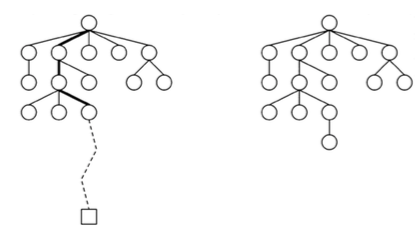
\includegraphics[width=.95\linewidth,height=2.0in]{images/basicprocess.png}
%\end{center}
%\caption{The basic MCTS process}
%\label{fig:BASIC}
%\end{figure}

%\begin{figure*}[!t]
%\begin{center}
%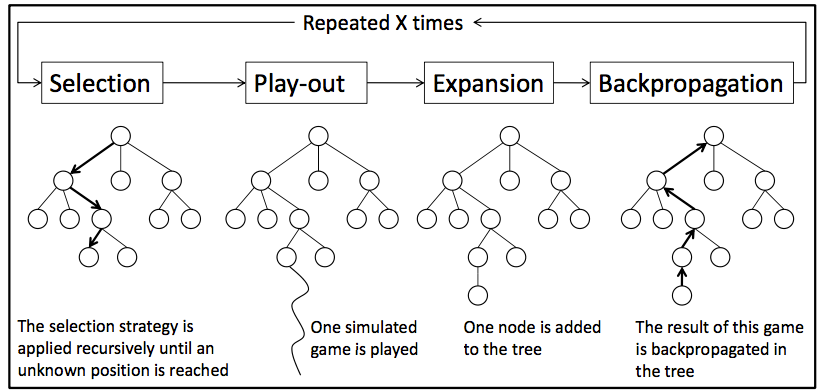
\includegraphics[width=\textwidth]{images/outlinemcts.png}
%\end{center}
%\caption{Outline of Monte-Carlo Tree Search (from~\cite{winands2010monte}) }
%\label{fig:OUTMCTS}
%\end{figure*}

% 2-col version in case we want it
%\begin{figure*}[!t]
%\begin{center}
%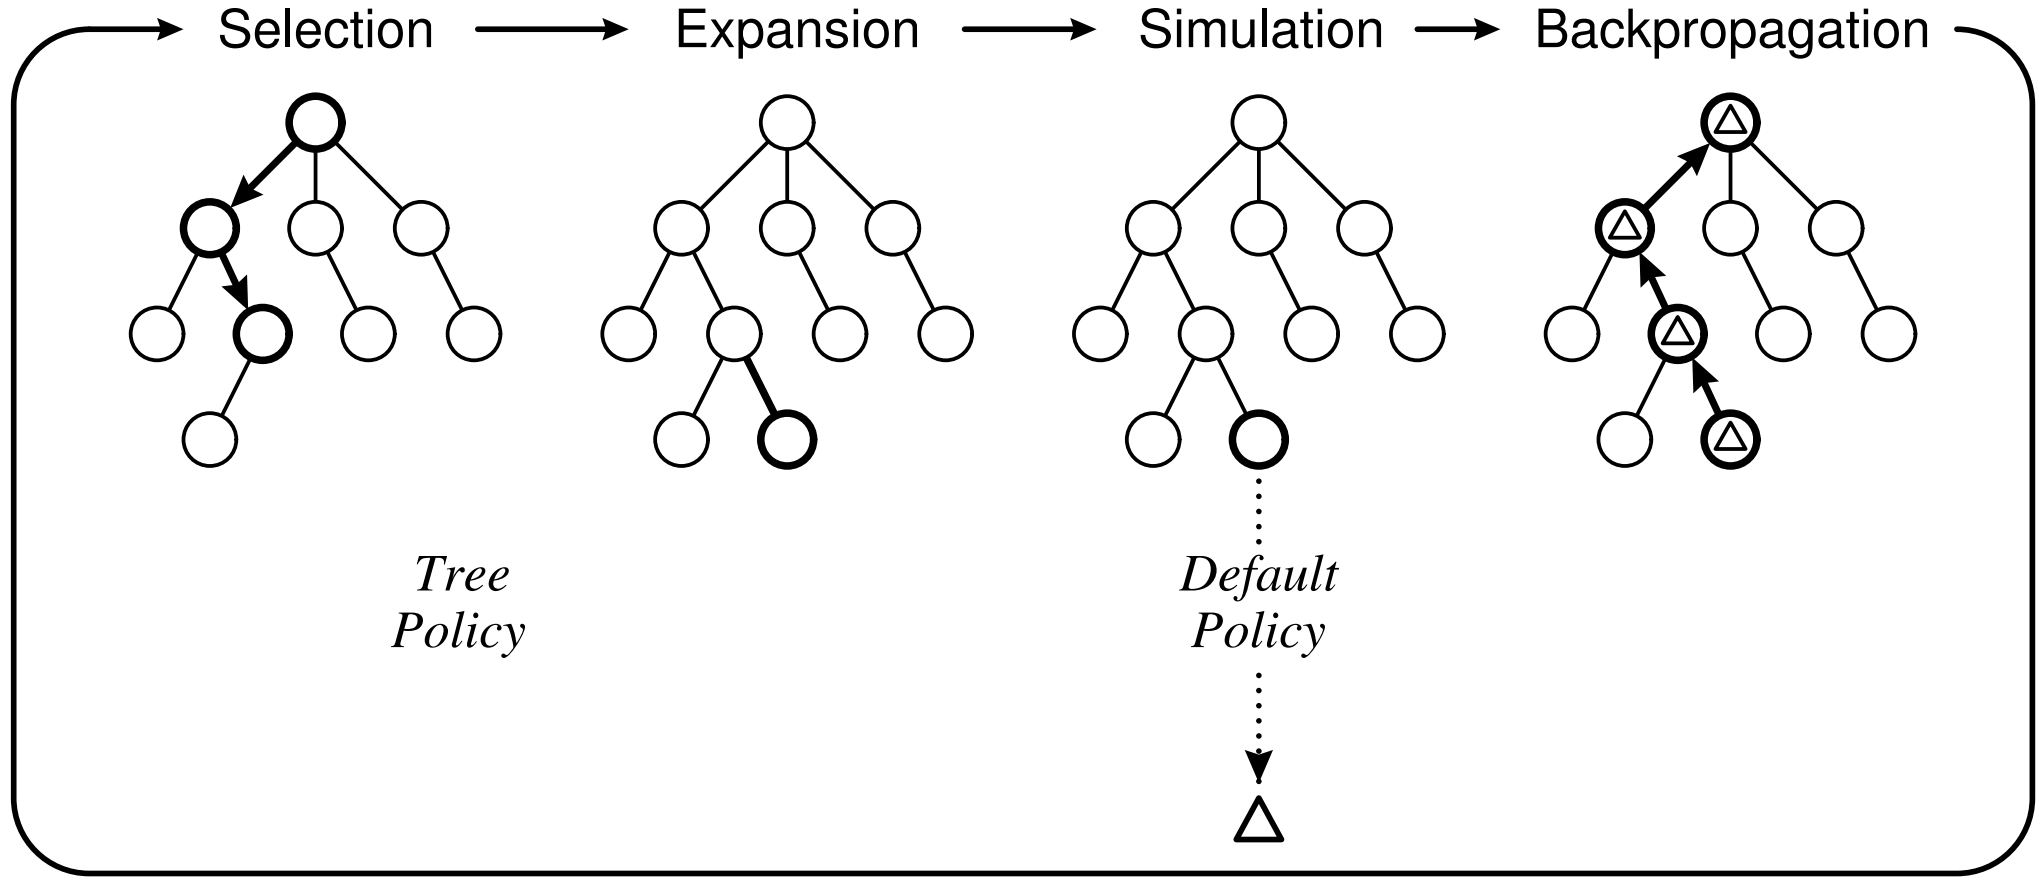
\includegraphics[width=\textwidth]{images/oneiteration.png}
%\end{center}
%\caption{Outline of Monte-Carlo Tree Search (from~\cite{browne2012survey}) }
%\label{fig:OneIter}
%\end{figure*}

\begin{figure}[b]
\begin{center}
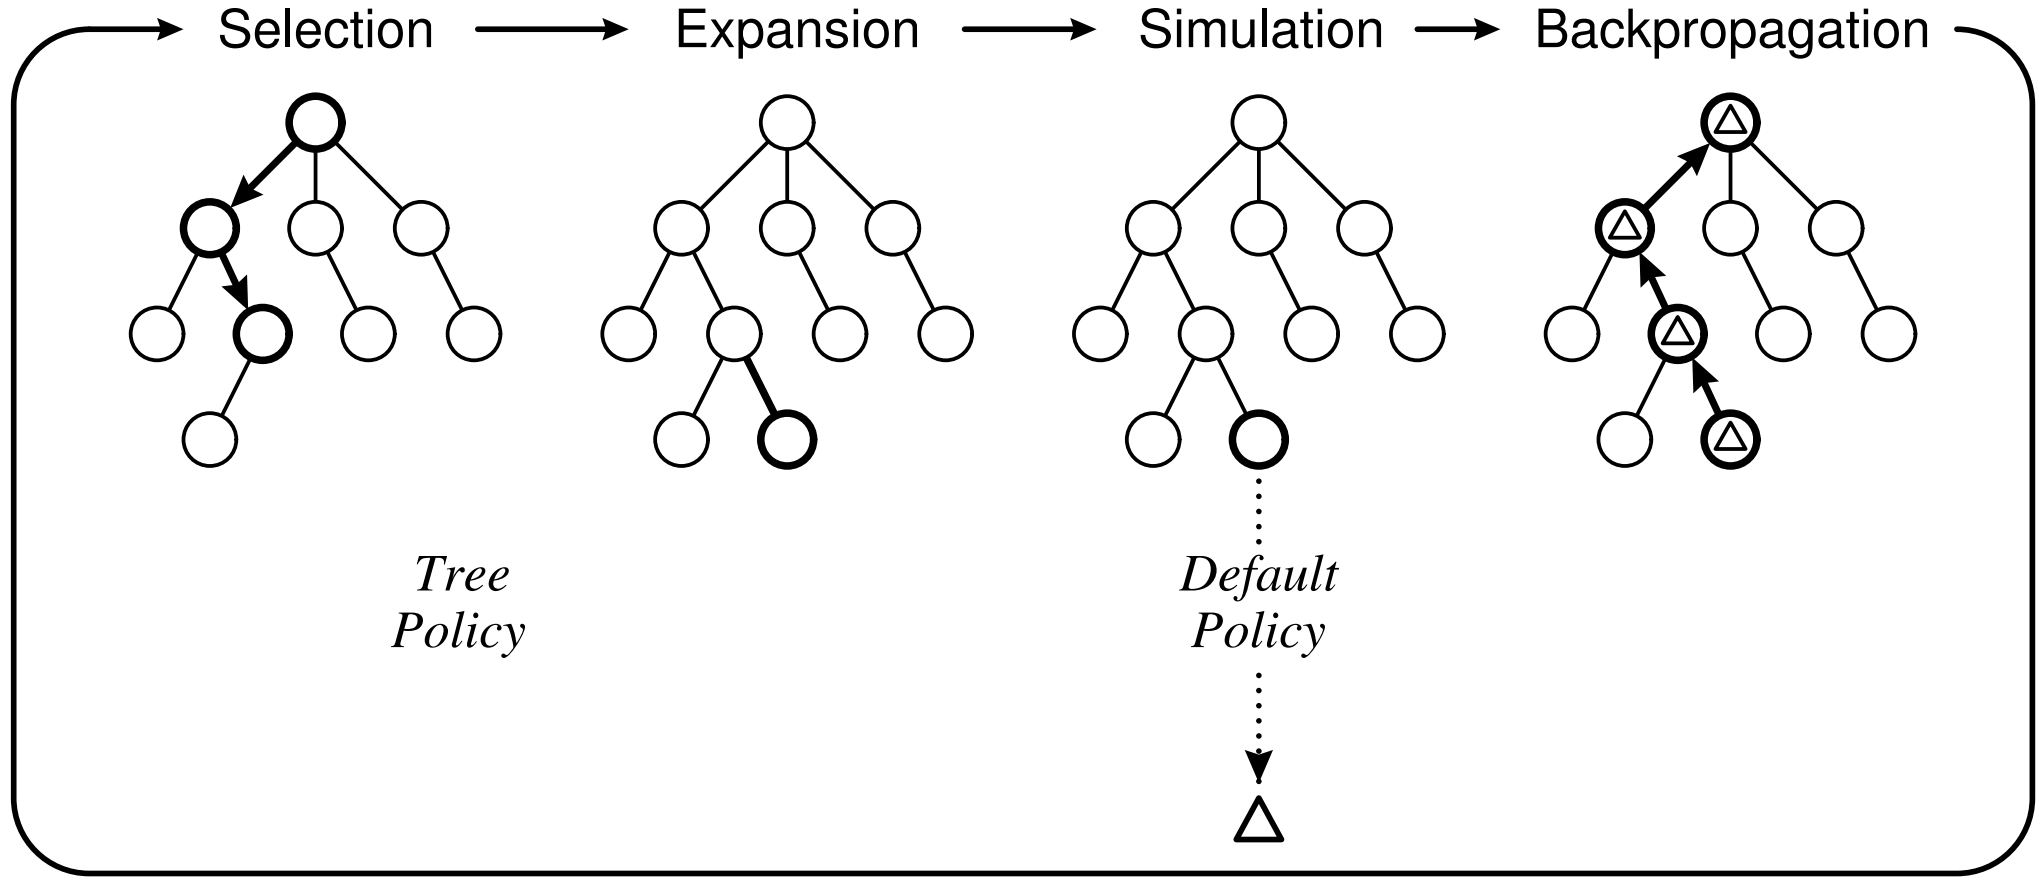
\includegraphics[width=.95\linewidth]{images/oneiteration.png}
\end{center}
\caption{Outline of MCTS~\cite{browne2012survey} }
\label{fig:OneIter}
\end{figure}

%{\bf SAB I made a new screen shot of this image to make it clearer, so please make sure you've updated yours with what I send here. (The trick is to zoom in as much as the monitor will allow before taking the shot.) I'm still not 100\% sure we can just take the image, but we'll do that for now...}

Like other game playing algorithms, at its core MCTS involves the creation of a game tree to decide on a move. MCTS is typically applied to games with extremely large trees, because the algorithm is designed to build the tree selectively rather than exhaustively. This is based on a balance between further analysis of promising areas (exploitation) and moving into less-explored areas (exploration). Figure~\ref{fig:OneIter} summarizes the repeated four-stage process: selection, expansion, simulation, and backpropagation. The {\it selection} step balances goals of exploration and exploitation to determine a leaf node for further consideration. In {\it expansion}, a child of the selected node is created. In {\it simulation}, a game is played from that node to completion; in standard MCTS, this simulation game consists entirely of random moves. Finally, in {\it backpropagation}, the results of the simulation are used to update all nodes on the path from the selected node to the root. More specifically, each node's visit count $n$ is incremented, and each node's average score $Q$ is updated based on the result of the simulated game. In this way, the tree is gradually, and selectively, developed. Upon reaching some limit condition, a child of the root can be selected based on any of a number of criteria, such as highest $Q$ or highest $n$. For a detailed discussion of the MCTS algorithm, see~\cite{browne2012survey}.

%UCB1 is simple UCB policy noted by~\cite{auer2002finite} which has a logarithmic growth of regret divided by the number of visits.
%% RTA - commented to remove

%\begin{equation} \label{eq:UCB1}
%UCB1 = \overline{X}_j + \sqrt{\frac{2\ln{2}}{n_j}}
%\end{equation}

The upper-confidence bound extended for trees (UCT)~\cite{kocsis2006improved} defines the selection criterion \textit{RTA- by considering the value of visited nodes and identifying the highest valued one as a best move following principles of multi-armed bandit based search} {\bf SAB please fill in a sentence here}. Formally, UCT is defined as follows:

\begin{equation} \label{eq:UCT}
UCT = \overline{X}_j + 2C_p\sqrt{\frac{2\ln{n}}{n_j}}
\end{equation}

\noindent where $\overline{X}_j$ is \textit{RTA- the mean of the score or payoff of the branch's selection}{\bf SAB fill in*****}, $n$ is the number of visits to the parent node, $n_j$ the number of visits to child $j$, and $C_p > 0$ is a constant. Thus the $\overline{X}_j$ term is the exploitation term, through which nodes with higher average scores will receive higher UCT scores. Similarly, the second term is the exploration term, in which a child that has been visited significantly less frequently than the parent will receive a higher UCT score. Therefore, $C_p$ balances the calculation between exploitation and exploration.

As noted in the introduction, MCTS has been applied to a variety of game types and planning problems. PPS is a single-player game with uncertainty and randomness of selection. Most of the literature and research in MCTS has been for multi-player games. These typically resolve to a form of minimax or it's variation expectimax in zero-sum games. For single-player games the strategy is significantly different where a cumulative best score derived from a game's scoring rules determine better or worse resolutions. For games with uncertainty or `chance' it becomes necessary to virutalize an opponent scenario to accomplish the functionality of the multi-player game. This is done by creating two types of nodes, choice and chance. In the MCTS algorithm \emph{selection} uses UCT for choice nodes, but a random move is used for chance nodes. Although we did not do a complete implementation as proposed, \cite{schadd2012single} suggests a Single-player MCTS variation.

{\bf SAB The above paragraph is a good start - we just need more citations and quick summaries. For example, what papers on single player games did you read? What papers on stochastic multi-player games? Any stochastic single player games? Anything relevant about MCTS for card games in general, maybe? What lessons did these papers bring that apply to our work here?}

In general move pruning is a technique to remove sub-optimal moves from consideration with the goal of focusing attention on better scoring areas of the tree. A widely known pruning technique applied in multi-player games is $\alpha\beta$. General pruning strategies applicable to all MCTS are~\cite{browne2010monte}:
%RTA Having experimented with $C_p$ and concluded some possible reasons for it's lack of impact, pruning became a significant area of investigation. 
\begin{itemize}
\item \emph{Soft pruning} a node is created but identified as suboptimal to be dropped out of normal consideration but could be reevaluated for later inclusion and processing.
\item \emph{Hard pruning} node is not added to the tree for a given state thereby being removed from further evaluation.
\end{itemize}
Specific to UCT, \cite{huang2010pruning} proposes two strategies based upon visit counts: \emph{Absolute pruning} all except the most visited and \emph{Relative pruning} attempts to detect when the most visited will remain so.

{\bf SAB: Nice stuff above. We may work with that more in a bit. Can you do something similar for simulation enhancements? And also domain knowledge? Maybe Cp adjustments?}

\textit{RTA: Additonal pruning strategies using heuristics for the multi-player card game Lords of War are found  in~\cite{sephton2014ieee}. Discussed were state evaluations and the relevance in making pruning decisions. Consideration of the time involved in the evaluations, i.e. effeciency, must be weighed against the potential loss of tree exploration. Significant increased levels of competitiveness were gained by considering the moves which were possible from a given state and incorporating card counting.}

\textit{RTA: MCTS incorporated into a Lines of Action (LOA) player was proposed by~\cite{winands2010monte}. LOA is a multi-player strategy board game in which an improved result was gained with simulation strategies. It is not uncommon to skip MCTS with the last one or few moves in conjuction with or in place of an evaluation cut-off. Normally MCTS is allowed to run to terminal state or leaf node which triggers backpropagation. Proposed instead was an earlier triggering if evaluation satisfied a threshold requirement.}

\textit{RTA: ~\cite{maes2012monte} proposes a generalizable approach in the application of Monte-Carlo Search (MCS) to new problems with single-player games. They suggest a language scheme for use in automatic discovery of MCTS algorithm components for use in multi-armed bandit development. By giving each element of MCTS like UCT, look-ahead, selection, and regression developed by the research of others, they define a formal method of retrieving components necessary to solve your a problem.}

\textit{RTA: The size of our game space is calculated as $\frac{52!}{27\times26}$ or $1.12 \times 10^{65}$. MCTS constructs very large trees and as surveyed in~\cite{browne2012survey} may be well suited to parallelization and\/or multi-threading. Several techniques are possible such as parallel tree simulation where multiple trees are processed simultaneously. A possible drawback to this approach is that since each thread uses a copy of the same tree they may traverse similar or even identical parts of the tree. Root parallelization initiates each thread with the same beginning root but then builds independant trees. A possible advantage here is that each thread may run to a limit and stop at any time idependantly. }

% RTA - commented
%Rather than base a pruning strategy on the visited count our focus was on estimated board score, or accumulated hand scores, at a given node which could be considered \emph{domain knowledge}. This was a hard pruning strategy because if a node was estimated to fall below a given threshold it would not be added to the tree. We had to be careful of over-pruning leaving no nodes available for selection or simulation and crashing the algorithm. This was accomplished by using a retention policy. This helped us to eliminate weaker positions and improve our player's scores.
%
%Another improvement to our player's scoring was accomplished with the implementation of a modified simulation strategy. Standard MCTS suggests choosing a child node at random and running simulations from this child. We were able to improve our scores consistently by choosing the child node with the best estimated board score.
%
%{\bf SAB: We can't really say "many of the available papers" without also citing specific examples and explaining briefly what they do. The explanation for each paper may be part of a sentence, up to a few sentences, in length.}
%
%Many of the available MCTS papers discuss with varying degrees of specificity application of domain knowledge as enhancement of MCTS. Our initial implementation of the algorithm followed the model of updating $Q$ and $n$ in the \emph{backpropagation} after a simulation. $Q$ is the calculated board score of a full board of 25 cards based upon the active scoring system. With the objective of elevating our player's final game scores, we developed a system of interim board evaluation calculating an estimated hand score for each row and column containing one to four cards. Once five cards are present this value is no longer an estimate. All of the possible hand types were determined and for one to three card an a-priori probability was applied while once four cards where present then card counting was employed with it's resultant probabilities. To maintain the exploration/exploitation MCTS balance, an increasing weighting factor was applied.
%
%{\bf SAB: Again, what literature specifically? What can you say specifically about each of a few selected papers relevant to the topic of this paragraph?}
%
%Some of the literature suggested positive results with multi-threading MCTS while others saw no impact. We tested a four thread player anticipating a modest increase in the number of trials accomplished. As noted by ~\cite{browne2010monte} to realize a $2X$ increase in score a $10X$ increase in the number of trials completed might be required. Our threaded player only improved on trial counts a little over $2X$ with no statistically viable improvement in score.

%%%%%%%%%%%%%%%%%%%%%%%%%%%%%%%%%%%%%%%%%%%%%%%%%%%%%%%%%
\section{Parameterized Poker Squares}

Poker Squares is a single-player card game played on a 5 x 5 grid. The player draws one card at a time and must determine where to place that card in the grid. Once placed, a card may not be moved. The object of the game is to create as many high-scoring poker hands as possible in each of the five rows and five columns. Due to the overlapping of rows and columns and the uncertainty of what cards will be drawn in what order, players must balance the risk of attempting high-scoring hands with taking more easily-attained hands.

Two scoring systems are most common in human play: American and British. Table~\ref{tbl:scoring} lists the hand values for each. Most rule books suggest that a game score of 200 for American or 70 for British is considered a ``winning'' result.

The ``parameterized'' part of the game name comes from the added challenge that the player is not told the scoring system until the moment the game begins. So the scoring system may be standard American or British, or perhaps a system in which positive points are given for a full house and negative points for all other hands, or even a random scoring system as in the last column of Table~\ref{tbl:scoring}.

%%%%%%%%%%%%%%%%%%%%%%%%%%%%%%%%%%%%%%%%%%%%%%%%%%%%%%%%%
\section{MCTS Application to Parameterized Poker Squares}
{\bf RTA Ready for review}

\begin{table}%[b]
\caption{American, British, and a random scoring system}
\label{tbl:scoring}
\centering
\begin{tabular}{c c c c}
\hline
Hand & American & British & Random \\
\hline
royal flush     & 100 & 30 & -23 \\
straight flush & 75 & 30 & -55 \\
4 of a kind    & 50 & 16 & 32 \\
straight        & 25 & 10 & -64 \\
full house     & 20 & 5  & -102 \\
3 of a kind   & 15 & 12 & 16 \\
flush           & 10 & 6   & 118 \\
2 pair         & 5   & 3   & -126 \\
1 pair         & 2   & 1   & 11 \\
high card    & 0   & 0   & -128 \\
\hline
\end{tabular}
\end{table}

%\begin{table}
%\caption{Scoring Systems: Ameritish and a random.}
%\label{tbl:SSATRD}
%\centering
%\begin{tabular}{c c c}
%\hline
%Hand & Ameritish & Random \\
%\hline
%royal flush & 47 & -23 \\
%straight flush & 47 & -55 \\
%4 of a kind & 24 & 32 \\
%straight & 13 & -64 \\
%full house & 9 & -102 \\
%3 of a kind & 8 & 16 \\
%flush & 6 & 118 \\
%2 pair & 4 & -126 \\
%1 pair & 1 & 11 \\
%high card & 0 & -128 \\
%\hline
%\end{tabular}
%\end{table}

%RTA mod Our MCTS implementation of PPS is built on top of the code in~\cite{hughart2012uct}, used under the MIT software license. 

Our MCTS implementation for PPS is built on the code in~\cite{hughart2012uct}, and used under the MIT software license. This section outlines various modifications made to the core MCTS algorithm, including the addition of PPS domain knowledge.

{\bf SAB: Still needs to be done}

%{\bf SAB: }Standard MCTS with chance and choice nodes. We used "equation 1"   backslash ref brace  closebrace   . Refer back to whatever equation is in the related work section, being explicit that that's what we did.

%{\bf SAB: }Start with the 5-card score, how it's computed 10 times for the board. This is sufficient for the core MCTS algorithm - all you need is the final score. Q value.

\subsection{Core MCTS}

Our implementation of the algorithm adhered to equation \ref{eq:UCT} following the model of updating $Q$ and $n$ in the \emph{backpropagation} after a \emph{simulation}. $Q$ is the calculated board score of a full board of 25 cards, or 10 5-card hands, based upon the active scoring system. Given the game's time constraint, knowing that 25 moves are necessary to fill the board, 30 seconds was divided evenly across each move. Simulations were executed until the move's time expired which fulfills core MCTS requirements. Our initial expansion created 25 empty choice nodes and randomly selected one in which to play the dealt card then expand the next level of tree and run simulations. Results of these simulations when then inform the placement of the next dealt card iteratively until completion of the game.


%{\bf SAB: }Pruning - remove children that are "clearly bad", but recognizing we just have an estimate, a heuristic, so not just always taking the "best", because our board evaluation is not going to be 100\% accurate, and we have uncertainty! So we need an heuristic. Lots of domain knowledge.
5 cards: we know exactly.
4 cards: describe the awesome stuff you guys did. 0-1-2 array, the probabilities
1,2,3 cards: multipliers
how 0 cards is rated
So, with that heuristic, how is it used for pruning? Have to get at least some constant times the parent score, but then to avoid pruning everything in some cases, if below 30% of children, then take all above average... Pruning happens for both selection and simulation stages. Pruning only happens on choice nodes.

%{\bf SAB: }Another way to modify the system: what does simulation look like? Using the heuristic to make a decision for choice nodes, still random on chance nodes.

\subsection{Hard Coding}

%{\bf SAB: }Hardcoding of first couple and last couple moves, equivalence classes of moves

%{\bf SAB Explain briefly how this saves time.}

An early change was the implementation of hard coded moves. By this we mean moves where, due to the limited number of effectively different moves that can be made, MCTS does not need to be run in order to make a decision. For example, the very first move of the game. Due to how Poker Squares (PS) is played, the very first move of a game does not have any bearing on the potential score of the board. No matter where the first card is played, it takes up a space in one row and in one column, and nothing else. Therefore, we elected to save time for moves where MCTS would be more useful by always placing the first card drawn in the upper left hand corner of the game board. By saving time we mean that since only milliseconds are required to place a card and calculate it's impact on the board (as explained below) this move's allotment of the available 30 seconds is given to later moves. Similarly, in the 2nd move of the game, the 24 remaining open spaces can be simplified into two equivalence classes of moves : the first is to play the new card in the row or column containing the first card played, and the second is to play it in a different row or column, so it begins to build a hand separately from the first. Then only a quick calculation is needed in order to determine which of those options is preferable - saving a lot of time, and eliminating the redundancy of checking moves that will ultimately have the same effect on the board. Additionally, this calculation allowed us to begin to have more control over the MCTS decision making process, instead of just evaluating purely randomized end-game boards.

Similarly,  we also looked towards the end of the game for moves to simplify. The 2nd to last move only has two relevant moves - the difference being that this time, they’re the only two moves at remaining to complete the game. While MCTS is capable of distinguishing between these moves, we decided to use a calculation similar to that of the 2nd move in order to allow for more time for MCTS in earlier moves. Finally, we hard coded the final move of the game. There is no need for any kind of decision making for this move, as there is only one possible option left on the board.

\subsection{Heuristics}

With the objective of elevating our player's competitiveness, we developed a system of interim board evaluation calculating an estimated hand score for each row and column which contained one to four cards. Using heuristics in the simulation step biased MCTS towards more reasonable plays resulting in significant increases in performance. Due to the variety of options for scoring systems in PPS, we lose the ability to include a rating for which poker hands are the most optimal to make. To compensate this, all of the possible hand types, from high-card to royal flush, are determined and tracked  as '0' for no longer possible, '1' still possible to make, and '2' already made.  For one to three card an a-priori probability was applied which was derived from standard poker statistics. Once four cards where present then we employed a card counting heuristic assessing what was already played on the board and how many moves remained with its resultant probabilities. When five cards are present this value is no longer an estimate and processed as described above. With this, we calculated a probability for being able to finish any of the remaining possible hands in a given row or column. For example, if you had the Ten, Jack, Queen, and King of Hearts in the topmost row, then the chance of you finishing that hand into a royal flush in the next draw is the chance of drawing the Ace of Hearts from what remains. Alternatively, you could also finish the hand into a flush by playing any of the six Hearts cards that won’t finish the hand into a Straight or Royal flush. A potential issue with this approad is that if there is more than one move left in the game, then taking only the chance of drawing a specific card in the next draw seems inaccurate. However, trying to use a combinatorial equation to determine the chance of drawing it before the end of the game assumes that you draw all of those cards at once, which is also not how this game is played. Since neither option seemed to increase the realistic accuracy of our algorithm, we went with the option that was less intensive to calculate.

We then add the scores of each of the possible hands remaining (each weighted by its calculated probability) together to get an expected value for that hand. These scores are able to vary from point system to point system, giving our player flexibility in which hand types it tries to prioritize, so if a pair or even high card ends up being more valuable than a flush or full house, the player can properly prioritize which hand types it should be attempting to make. Due to the heavy computational strain of calculating an expected value for only four cards, and the fact that the calculations would only be more intensive for a hand with fewer cards in it (as there are more cards that need to be filled in, and more work would need to be done to determine what cards are missing, and it would take multiple draws to finish the hand), we decided to move away from calculating an explicit expected value for hands with fewer that four cards. Instead, for hands below four cards, we use an estimated value. Still calculating what hands are able to be made, but instead of calculating the probability of drawing the cards necessary to finish each of those hand types, we weight the score of each hand with an a-priori probability of being able to finish that type of hand. We calculated these a-priori values using the British scoring system for Poker Squares, which is said to be based on the difficulty of finishing each of the hands in a game of Poker Squares. We found that this mixed approach to calculating scores balanced estimated accuracy with computational intensiveness. Once each row and column has a value, they are all added together to create the board as an estimated value. This value can then be compared between siblings, and decisions can be made based on which children look the best. 

Another improvement to our player's scoring was accomplished with the implementation of a modified simulation strategy. Standard MCTS suggests choosing a child node at random and running simulations from this child. We were able to improve our scores consistently by choosing the child node with the best estimated board score.


\subsection{Pruning}

%{\bf RTA: Copied from related work}
Rather than base a pruning strategy on the visited count our focus was on estimated board score calculated as described above. This was a hard pruning strategy because if a node was estimated to fall below a given threshold it would not be added to the tree. A score for each state was determined and a mean calculated of all the children. If a child's score did not exceed a threshold then it was not added to the tree. However, to avoid overpruning, there was a pruning limit which controlled the percentage of pruning allowed. This helped us to eliminate weaker positions and improve our player's scores.


%%%%%%%%%%%%%%%%%%%%%%%%%%%%%%%%%%%%%%%%%%%%%%%%%%%%%%%%%
\section{Experiments and Analysis}

%-----------------------------------------------------------------------------------------------------------------------------------------------------------------
\subsection{The Exploration--Exploitation Tradeoff}
Recall from equation (\ref{eq:UCT}) that MCTS with UCT attempts to balance the {\it exploitation} of relatively effective paths with the {\it exploration} of lesser-known paths. This balance is controlled via the constant $C_p$, where a higher value means a stronger emphasis on exploration. As discussed previously, ~\cite{kocsis2006improved} suggest that $C_p = \frac{1}{\sqrt{2}}$ is ideal when rewards range in $[0,1]$. 

A rewards range of 0 to 1 is simple when applied to a 2 player game. 0 can represent a loss, and 1 can represent a win. However, because Poker Squares is a single player game, success is measured based on an end-of-game score instead of on whether or not the game was won. Depending on the scoring system, final scores could be in the high hundreds, entirely negative, or anywhere in between. 

Due to the importance of the scoring sytem in setting an optimal  $C_p$ value in UCT, we created a score squashing algorithm that normalized the minimum and maximum potential board scores of a scoring system to 0 and 1. We tried two methods of squashing. The first calculated a highly accurate minimum and maximum score, taking into account the fact that certain hand types can only be made a certain amount of times. For example, in the American scoring system, Royal Flushes have the best score. But you can only make four Royal Flushes on the same board, so it fills in the remaining possible hands with the best scoring moves that are still possible. Once four Royal Flushes are placed (they must all be parallel, so either all four must be in rows or all four must be in columns), a Straight Flush can be placed in the fifth row or column, but no more variations of straights or flushes can be placed on this board. So the final five hands are filled with the next best scoring hand, Four of a Kind, for a final score of 725. The minimum score in the American System is easy - it is possible to only have a high card hand in all rows and columns, so the minimum possible score is 0. 

This method is computationally expensive to calculate, so we also created a less accurate but much faster method of calculating a minimum and maximum - take the lowest hand score and multiply it by ten for the minimum, and multiply the highest by 10 for the maximum. This results in a range of 0 - 1000 for the American scoring system, which is wider than the precise calculation, but also much simpler to calculate. Additionally, we tested a squashing system that normalized 200 to 1, and another that normalized 2000 to 1, to determine how much imprecision in the normalization could affect performance. 

\begin{minipage}{\linewidth}
\centering
%\begin{table}
\captionof{table}{Effect of Score Normalization}
\label{tbl:SquashingTable}
%\centering
\begin{tabular}{c c c}
\hline
Player & Normalization Range & Mean Score \\
\hline
Precise Squashing & 0-725 & 91.36 \\
Imprecise Squashing & 0-1000 & 91.23 \\
Max 200 & 0 - 200 & 90.12 \\
Max 2000 & 0 - 2000 & 89.54 \\
\hline
\end{tabular}\par
%\end{table}
\bigskip
Averages calculated over 1,000 games
\end{minipage}

These tests all used a  $C_p$ of $\frac{1}{\sqrt{2}}$. As mentioned previously, this has been shown to be the ideal  $C_p$ value using ranges between 0 and 1.

The results in Table~\ref{tbl:SquashingTable} show that the range normalized to between 0 and 1 has little effect on performance.

We then tested various $C_p$ values on the American scoring system to determine what an optimal $C_p$ value would look like without squashing, and how different $C_p$ values affect player performance.

\begin{figure}
\begin{center}
\begin{tikzpicture}
\begin{axis}[width=.95\linewidth,    % was axis
	xlabel=$C_P$,
	ylabel=Mean Score, 
	axis lines=left,
	%xtick={0.00, 5.00, 10.00, 25.00, 50.00},
	xmin=0, xmax = 60,
	ytick={30.00, 60.00,90.00,120.0},
	ymin=0, ymax = 100,
	scaled y ticks = false,
	y tick label style={/pgf/number format/fixed}]
\addplot [only marks, mark size=1pt] table[y=mean_value, x=cp]{data/cpexperiment.dat};
\end{axis}  % was axis
\end{tikzpicture}
\end{center}
\caption{$C_p$: Effect of $C_p$ on Mean Score, no Squashing.}
\label{fig:CPEXP}
\end{figure}

$C_p$ values were tested by running 700 games per value under the American scoring system. These experiments were done with a simple MCTS implementation; no domain knowledge was applied in selection or simulation. 

In our experiment shown by Figure~\ref{fig:CPEXP}, higher $C_p$ values  led to better results, up until further increases leveled off in effectiveness. It seems that dividing the searches as evenly as possible between siblings (nodes at the same level, as possible choices of progressing the game from its current state) led to the best results, which would explain why anything higher (which would not change anything significant, as exploration is already weighted far more heavily than exploitation) had no significant effect. So we fixed our $C_p$ value at the lower bound of this effectiveness plateau.

Additionally, by comparing Table~\ref{tbl:SquashingTable} with Figure~\ref{fig:CPEXP} you can see that the squashing values with a  $C_p$ of $\frac{1}{\sqrt{2}}$ performed at the same level as the best scoring  $C_p$ values with no squashing algorithm. 

%Note - should we run more tests with different scoring systems and $C_p$ values in order to see the specificity of our current weight
%
%{\bf SAB: Do we also want to include experiments about other scoring systems. We have a little bit of data already with a random scoring system.}
%
%{\bf Note:} If we can say that our $C_p$ value should change based on the scoring system, we can go back to squashing down to 0-1 and use $\frac{1}{\sqrt{2}}$, that way we can back up our decision by quoting the Brown paper and claiming to fulfill the Hoeffding inequality.
%
%If we can say that our $C_p$ value does not need to change, we would have to look more into the significance of $C_p$ values as stated by other papers, because so far other papers have said that a good $C_p$ depends heavily on the range of scores in use, so we could either dispute that or figure out why it is different for us (the chance nodes? The size of the game space? Go’s game space is even larger than ours, though I can’t recall reading about MCTS Go and $C_p$ values)

%{\bf possible tests:} run our code with a way higher (or a significantly lower) scoring system, see if it imbalances our $C_p$ value. If it does, follow up with another squashing experiment.

%{\bf SAB: May just need to say that since we didn't see a big difference in preliminary experiments, we didn't explore it further, but there could be more to explore in future work.}

%-----------------------------------------------------------------------------------------------------------------------------------------------------------------
\subsection{Hardcoding Certain Moves}

As discussed in section (****related work****), many researchers have found great benefit in the application of domain knowledge to MCTS. Section (****MCTS Application to parameterized poker squares****) describes two types of domain knowledge used in PPS in this work. The first application is the implementation of hard-coded moves, or moves that skip MCTS in favor of a faster calculation.

Overall, hard coding saved us 4 moves worth of time, resulting in a 19\% increase in time for each of the remaining moves over the non-hard-coded player.
	
%(calculation done by 4/25 = .16 ( 16\%of the total time allowed), .16/21 = .007 (each move gets an additional .7\% of the total time allowed), 1/25 = .04 (how much of the total time allowed each move gets), .007/.04 = .19 (adding the .7\% of the total time increases an individual move’s time by 19\%)

Considering that our player can run tens of thousands of simulations in a second (we may want to be more precise here, at least lay out that result somewhere), even an increase of a fraction of a second can give the decision making algorithm at that level significantly more information to make an informed decision with.

Even with four moves worth of time saved, we saw an almost negligible change in score. Allowing for other moves to have more time to run MCTS lets them make more informed decisions, but due to the large game space the extra time given by the hard coding only allows a small percentage of the possibilities at any individual move to be further explored, so the score increase for each hard coded move remains small. Our player’s average score improved by 1\% due to the 4 moves of hardcoding. Because hard coding saved computation time and at the very least did not decrease our score, we decided to maintain that change, but not explore the potential of further hard coding.

%-----------------------------------------------------------------------------------------------------------------------------------------------------------------
\subsection{Domain Knowledge and Simulation}

%fixed: Simulation improvement using domain knowledge, but no pruning in selection
%variable: totally random simulation versus just choose the best move 
%result: choose best move is better

The second type of domain knowledge we applied was the creation heuristic evaluation of the game board to be used during the simulation step of MCTS. To determine the effectiveness of a heuristic simulation, we tested a player that did not utilize domain knowledge against a player that used the heuristic discussed in section (****Developing a Parameterized Poker Squares Heuristic****) in its simulation step. 

Using the heuristic during simulation instead of randomizing moves resulted in a significant increase in score. The best improvement in performance came by only allowing simulations to run with the best-looking child given by our heuristic. 

As shown by Table~\ref{tbl:SimulateTable}, using a heuristic to improve the strength of simulations resulted in an average score increase of 45\% over our no-domain-knowledge player.

%{\bf We could also note from our data that our heuristic player had a better minimum and maximum scoring board state, if we thought that could be relevant enough to mention}

\begin{minipage}{\linewidth}
\centering
%\begin{table}
\captionof{table}{Effect of Domain Knowledge on Simulation}
\label{tbl:SimulateTable}
%\centering
\begin{tabular}{c c}
\hline
Player & Mean Score \\
\hline
No Domain Knowledge & 80.6 \\
Simulate With Heuristic & 117.8 \\
\hline
\end{tabular}\par
%\end{table}
\bigskip
Averages calculated over 10,000 games
\end{minipage}

%-----------------------------------------------------------------------------------------------------------------------------------------------------------------
\subsection{Domain Knowledge and Selection}

%fixed: Pruning in selection, with just some "sensible" weights
%variable: pruning just in selection with random sim vs. pruning in selection and simulation vs. pruning in selection and choose best sim.
%result: choose best move is better, and also we see the pruning in selection is helpful
%
%{\bf SAB: Remember, don't phrase things as a "play-by-play", as in: "After the effectiveness of our board evaluator at improving our player’s average score, we decided to apply a similar technique to the expansion step as well." Note alternative first sentence below.}
%
This set of experiments considers the application of the board heuristic to the selection step of MCTS. More specifically, when expanding a choice node of the tree, nodes scoring under a variable threshold with this heuristic were {\it pruned}. The expansion of chance nodes was left unaffected, as we do not get to decide which card we are going to draw. 

As discussed in section (****related works****), there are two typical strategies for pruning. Soft pruning tends to be more accurate over a longer period of time, as there is no risk of unintentionally permanently removing nodes that are more promising than the pruning algorithm makes them appear at first. However, due to the short amount of time each game is allotted, we elected to pursue a method of hard pruning instead.

When evaluating the children of a choice node for pruning, a scoring threshold is used to determine which children should be kept for consideration in MCTS and which should simply be pruned. This threshold is based on a percentage of the choice node's own score, so that moves that end up reducing the board's estimated value too far below the parent's get pruned first. In order to avoid overpruning (for example, if an undesirable card is drawn, and it does not fit well in any of the open spaces, so all of the children have lower estimated values), we implemented a minimum percentage of children that could be pruned. If the threshold algorithm pruned enough children that the percentage of unpruned children  went below our minimum, we would add back in any children above the average estimated values of all the children. We found that this method significantly reduced the size of the game space and did increase our player's average score, however the increase was not nearly as significant as the addition to simulation.

\begin{minipage}{\linewidth}
\centering
%\begin{table}
\captionof{table}{Effect of Domain Knowledge on Selection}
\label{tbl:SelectionTable}
%\centering
\begin{tabular}{c c c}
\hline
Selection Style & Simulation Style & Mean Score \\
\hline
No Domain Knowledge & No Domain Knowledge & 80.6 \\
Pruning & No Domain Knowledge & 88.9 \\
No Domain Knowledge & Heuristic & 117.8 \\
Pruning & Heuristic & 120.1 \\
\hline
\end{tabular}\par
%\end{table}
\bigskip
Averages calculated over 10,000 games
\end{minipage}

One possible reason for this disparity is due to the number of simulations that are run compared to the number of times a node is expanded. According to our calculations, our player averages about 10 simulations per expansion. (a number given by our tracking of num pruned nodes) 

Another possible reason is that, while simulations direct MCTS into which nodes are most valuable, it does not eliminate any nodes from consideration. Pruning in the expansion step, however, could potentially remove play options that aren’t actually suboptimal, due to the imprecise nature of estimated values and imperfections in our calculation.

%-----------------------------------------------------------------------------------------------------------------------------------------------------------------
\subsection{Further Tuning of Domain Knowledge}

%fixed: pruning in selection, choose best move for simulation
%variable: the weights for the board score
%result: the best weights we came up with

 %Once we decided to keep our pruning algorithm, we ran a series of tests meant to determine what values for constants in our equation gave the best average results. When we ran tests for our potential different weights, our highest scoring test increased its score 20\% over the lowest scoring test (sheet four in our results). This shows how important an accurate method for pruning is. 

\begin{table}
\caption{Results of experiments on heuristic parameters}
\label{tbl:heuristicParameterResults}
\centering
\begin{tabular}{c c c c c c}
\hline
Mean & $\alpha$ & $\beta$ & $\gamma$ & $\beta : \alpha$ & $\gamma : \beta$\\
\hline
105.25 & 0.100 & 0.400 & 1.600 & 4.0 & 4.0 \\
109.07 & 0.050 & 0.400 & 0.600 & 8.0 & 1.5 \\
109.30 & 0.075 & 0.400 & 0.600 & 5.3 & 1.5 \\
\hline
109.89 & 0.125 & 0.400 & 0.600 & 3.2 & 1.5 \\
110.32 & 0.100 & 0.400 & 0.600 & 4.0 & 1.5 \\
111.94 & 0.500 & 0.500 & 0.700 & 1.0 & 1.4 \\
\hline
112.20 & 0.100 & 0.500 & 0.900 & 5.0 & 1.8 \\
112.81 & 0.200 & 0.500 & 0.800 & 2.5 & 1.6 \\
113.87 & 0.200 & 0.400 & 0.600 & 2.0 & 1.5 \\
\hline
114.49 & 0.300 & 0.500 & 0.700 & 1.7 & 1.4 \\
114.91 & 0.200 & 0.600 & 1.200 & 3.0 & 2.0 \\
115.14 & 0.150 & 0.450 & 1.350 & 3.0 & 3.0 \\
\hline
116.77 & 0.200 & 0.400 & 0.700 & 2.0 & 1.8 \\
116.95 & 0.125 & 0.250 & 0.500 & 2.0 & 2.0 \\
117.37 & 0.200 & 0.500 & 0.900 & 2.5 & 1.8 \\
\hline
118.72 & 0.050 & 0.200 & 0.800 & 4.0 & 4.0 \\
118.79 & 0.150 & 0.300 & 0.900 & 2.0 & 3.0 \\
119.42 & 0.050 & 0.150 & 0.450 & 3.0 & 3.0 \\
\hline
119.50 & 0.125 & 0.250 & 0.750 & 2.0 & 3.0 \\
119.66 & 0.200 & 0.400 & 0.900 & 2.0 & 2.3 \\
119.95 & 0.100 & 0.300 & 0.700 & 3.0 & 2.3 \\
\hline
119.99 & 0.150 & 0.300 & 0.600 & 2.0 & 2.0 \\
120.58 & 0.100 & 0.300 & 0.750 & 3.0 & 2.5 \\
120.75 & 0.100 & 0.200 & 0.750 & 2.0 & 3.8 \\
\hline
121.14 & 0.094 & 0.283 & 0.850 & 3.0 & 3.0 \\
121.60 & 0.075 & 0.150 & 0.500 & 2.0 & 3.3 \\
121.68 & 0.100 & 0.300 & 0.800 & 3.0 & 2.7 \\
\hline
121.99 & 0.100 & 0.300 & 0.900 & 3.0 & 3.0 \\
123.21 & 0.100 & 0.300 & 0.850 & 3.0 & 2.8 \\
\hline
\end{tabular}
\end{table}

\begin{figure}
\begin{center}
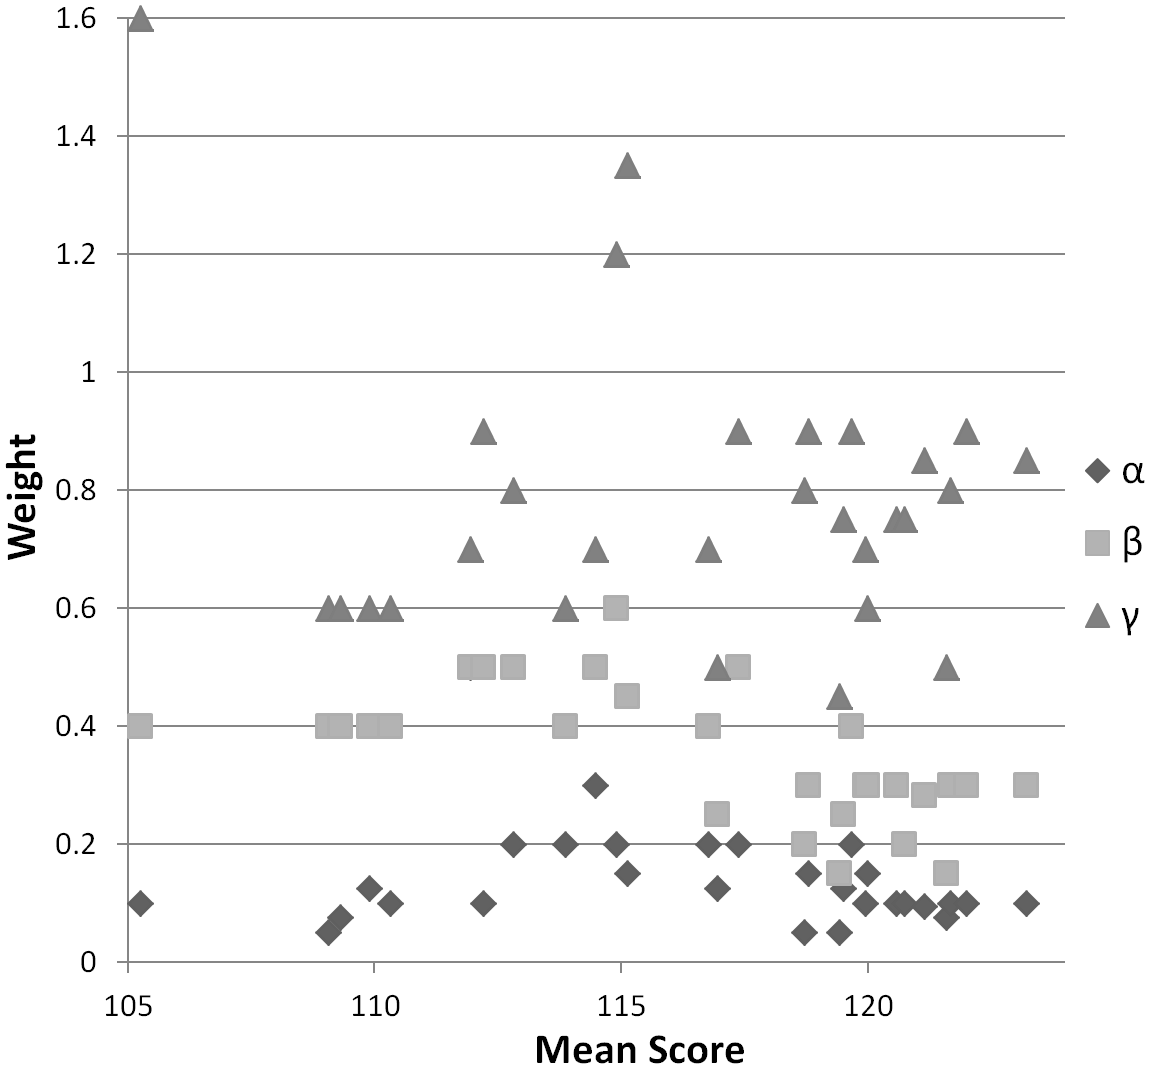
\includegraphics[width=1\linewidth]{images/1-2-3_weights.png}
\end{center}
\caption{$\alpha$, $\beta$, and $\gamma$ for each resulting mean score.}
\label{fig:123weights}
\end{figure}

\begin{figure}
\begin{center}
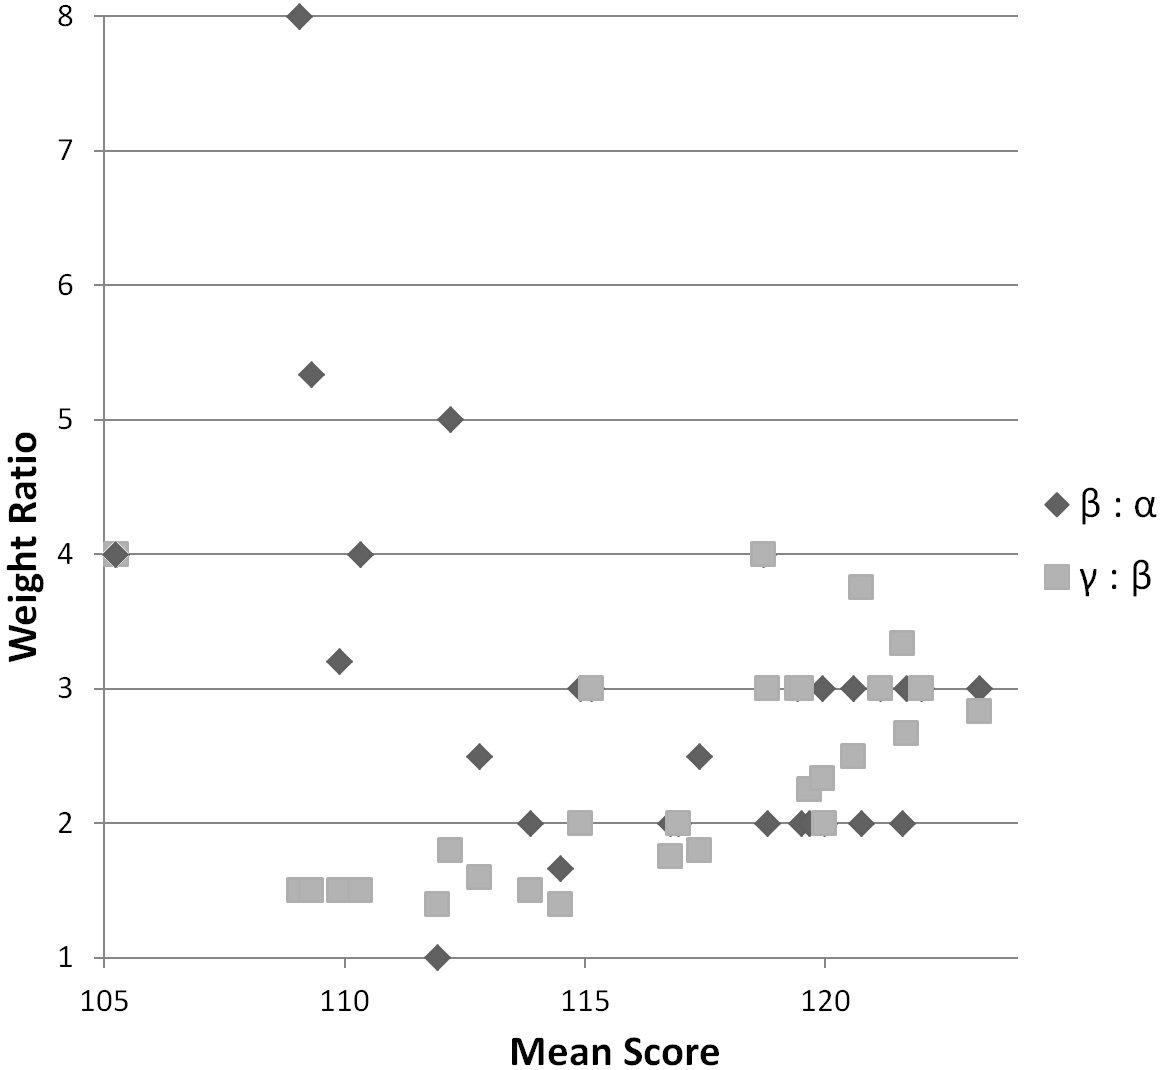
\includegraphics[width=1\linewidth]{images/1-2-3_ratios.png}
\end{center}
\caption{$\beta:\alpha$ and $\gamma:\beta$ for each resulting mean score.}
\label{fig:123ratios}
\end{figure}

The experimental results described so far show that some modifications have a very small effect, while others have a more significant effect. Recall in equation {\bf *****} that the heuristic includes parameters $\alpha$, $\beta$, and $\gamma$ for the weighting given to one-, two-, and three-card hands, respectively. Prior experiments used a ``reasonable'' guess for these parameters, or {\bf prior parameter values}. In this experiment, we examine these parameters more closely, with the system fixed at a $C_p$ value of {\bf *****}, hardcoding of starting and ending moves, simulation choosing the single highest-scored move (no randomness), and selection using pruning based on board score. These represent the best design decisions resulting from the previous experiments. The parameter settings considered further here have an influence on both the selection and simulation steps, as both depend on the heuristic.

Twenty-nine different trials were conducted for various settings of the parameters, with each trial involving several hours of game play. A few intuitive ideas were used to constrain the number of permutations considered. First, we ensured that $\alpha \leq \beta \leq \gamma$, since all else being equal, a hand with more cards is closer to completing any potential hands than one with fewer cards, and so it should be valued more highly. Second, the parameter space can be constrained somewhat by considering the ratios $\beta : \alpha$ and $\gamma : \beta$. This can bring new insights into what parameter settings may be more similar than would first appear by considering magnitudes alone, thus leading to hypotheses about what portions of the space should be prioritized for consideration. Having said this, however, recall that four-card hands are evaluated using an entirely different formula. So in fact the magnitudes of $\alpha$, $\beta$, and $\gamma$ do matter as well, rather than just the ratios, because hands with three or fewer cards will be compared not just among themselves but against four- and even five-card hands. So using ratios can be a useful analysis tool, but should not be used to the exclusion of considerations of magnitude.

Results of these experiments are shown in Table~\ref{tbl:heuristicParameterResults} and in Figures~\ref{fig:123weights} and \ref{fig:123ratios}, with the table showing the raw data used to generate the figures. Note that the table is sorted in order of increasing mean score, with values ranging from 105.25 to 123.21. For each mean score, the $\alpha$, $\beta$, and $\gamma$ values and the $\beta : \alpha$ and $\gamma : \beta$ ratios are provided. Visualization is challenging due to the presence of three independent variables, but some important insights can be gained from Figures~\ref{fig:123weights} and \ref{fig:123ratios}. In both graphs, note that the horizontal axis is the mean score, and vertical axis is the weight. Thus, the three shapes on the far left in Figure~\ref{fig:123weights} correspond to the values of $\alpha$, $\beta$, and $\gamma$ in the first row of the table. These are the parameter settings that led to a mean score of 105.25.

Note in both graphs that the results are fairly scattered on the left side where mean scores are lower, yet somewhat more uniform on the right side where mean scores are higher. This demonstrates a preference for certain parameter settings to obtain the highest scores. For example, in Figure~\ref{fig:123weights}, not only the single highest-scoring player, but nearly all higher-scoring players tend to have values around $\alpha = 0.1$, $\beta = 0.3$, and $\gamma = 0.85$, with stronger convergence in the $\alpha$ and $\beta$ values.

Figure~\ref{fig:123ratios} shows ratios. Recall that ratios are harder to work with because they ignore the magnitudes of the parameters, and thus the convergence is not quite as clear as in the parameter values themselves. Nevertheless a trend is visible, in which both a $\beta : \alpha$ ratio and $\gamma : \beta$ ratio of 2 or 3 is found in the highest-scoring players. Note that these ratios correspond well to the ideal parameter values already mentioned.

{\bf SAB ***** Make sure we address the different scoring systems - does system perform well with them?}
%%%%%%%%%%%%%%%%%%%%%%%%%%%%%%%%%%%%%%%%%%%%%%%%%%%%%%%%%

\section{whatevs}

Now we step back and look at bigger picture conclusions from the results, and theorize about why certain things were more effective than others.

Size of the game space in Poker Squares - 

Conclusion 1 - Continuing the tree search if the most visited root is not also the one with the highest reward has proven effective in some MCTS algorithms like the GO program ERICA (MCTS survey pg 8). However, this approach did nothing for our average score. We believe this to be because continuing to run MCTS on one move would take time away from subsequent moves, and due to our short amount of time with which to play this game reducing the time of later moves counteracted the benefit of continuing the search.

Conclusion 2 - Hard coding of moves. Some moves in Poker Squares can boil down to very straightforward decisions, which means you do not need to run MCTS on them, freeing up more time for other moves. This includes moves at the very beginning of a game, and moves close to the very end of one. At the start of a game, when there are only a few (or even no) cards on the board, the board can be simplified into equivalence classes of the effects a certain card placement could have. At the end of the game, the board is developed enough and each card placement location distinct enough that a decision making algorithm (like our pruning method, more on that later) can accurately distinguish between the moves without the need for MCTS.
	Very first move - 1 equivalence class (playing the first card has the same effect on the board no matter where it is placed)
	2nd move - 2 equivalence classes (either the second card is placed with the first, continuing to build one of those hands, or it is played apart from the first so that they do not interact)
	24th move (2nd to last, two spots remaining on the board) - it is very easy to tell what kind of effect a card will have on the board at this stage in the game, so use the decision making algorithm to determine which of the two spots is better
	25th (final) move - only one spot remaining, no need to do any decision making or MCTS.
We saw slight increases in score with each hard-coded move. Allowing for other moves to have more time to run MCTS lets them make more informed decisions, but due to the large game space the extra time given by the hard coding only allows a small percentage of the possibilities at any individual move to be further explored, so the score increase for each hard coded move remains small.
{\bf SAB: Setting aside the issue of occasionally running out of time, is there a score improvement when comparing using hardcoding (and therefore having more time for other moves) versus not using hardcoding? Or did it not seem to make a difference? Why do you think this is?}

Conclusion 3 - Multi threading. Having multiple (four) threads all running on/building the same tree gave us more MCTS trials overall, but did not result in a significant increase in score. Having multiple threads building separate trees and then comparing the results also gave more trials, but resulted in a decrease in score.
	Multiple threads on the same tree - having more MCTS trials did not help significantly because, although having more trials leads to more information about the game space, the game space of Poker Squares is so large that even a few million more trials does not have much impact. {\bf SAB: How large is the game space? Do we have an idea of what percentage of it can be considered by 1 thread, versus 4 threads? And how are you measuring percentage given that some nodes are visited many times in MCTS, while others are visited even just once?}
	Multiple threads with their own tree - running multiple threads seemed to reduce the individual efficiency  (less trials run in the same amount of time, so fewer nodes are visited and simulated from) of any one thread. {/bf SAB: What do you mean? Fewer nodes visited?} This isn't a major deal when running the threads on the same tree, as it does ultimately result in a significant net increase in overall trials. However, when each thread is running on its own tree and at reduced efficiency, each tree has less information on it, so the four best moves found can be less informed than in an individual thread running at higher efficiency. 

Conclusion 4 - discussed in conclusion 2 (hard coding)

Conclusion 5 - Cp values, balancing exploration and exploitation {\bf SAB: Yep, give some explanation of this. We should explain why it didn't seem to have much effect, perhaps in light of the size of the state space? Or something else too?}

Conclusion 6 - Squashing minimum and maximum values for a scoring system in order to keep consistency between them{\bf SAB: May need to discuss this in the MCTS Application to PPS section. What was done... Then if there are any interesting results to discuss about this step specifically here, we can include them.}

Ran a test tournament (tourney3) with multiple versions of player (and a depth2 greedy player as a baseline), each with a different C value for the UCT formula. player 1 has a C value of $\frac{1}{\sqrt{2}}$, player 200 has a C value of $\frac{200}{\sqrt{2}}$, and player 725 has a C value of $\frac{725}{\sqrt{2}}$. At the time of tourney3, the UCT formula code was as follows: 
{\bf SAB: These kind of formulas would be earlier in the paper, like in MCTS Application to PPS section. The different cp values used would be described in the results section. In analysis, here, we'd explain *why* the results worked out in the way they did.}

{\bf SAB: We should make this a little less code-like. No "get", no "Float.MIN\_VALUE". Also, use $log_{10}$ - note the braces grouping the 1 and 0 together as subscripts, compared to $log_(10)$ which makes only ( a subscript. And the tiny command probably isn't a good idea. We just need shorter variable names, but not so short that their meaning isn't fairly clear.}

\tiny
\begin{equation}
{nodeScore =  \frac{getScore}{getTimesVisited + MIN\_\\VALUE} } \label{eq:sq}
\end{equation}  
\normalsize

\tiny
\begin{equation}
{bias = 2 * C * \sqrt{\frac{log_(10) curNode.getTimesVisited}{curChild.getTimesVisited  + Float.MIN\_\\VALUE}}} \label{eq2:add}
\end{equation}  
\normalsize

\tiny
\begin{equation}
{randomizer = MIN\_\\VALUE * Random\left(nextMoves.size^2\right)}        
\end{equation}  
\normalsize

\tiny
\begin{equation}
{biasedScore = nodeScore + randomizer + (bias)}
\end{equation}  
\normalsize

Evaluated our output at numerous locations in the code, focusing on the selection, expansion, and simulation steps, particularly in regards to how they each handle card decks.
In order to modify our UCT code, we could: 
Try different formulas, keeping our constants and scoring system the same
Try different constants, keeping our formula and scoring system the same
Try different scoring systems (squash the scores), keeping our formula and constants the same
Then mix and match different options until we find something that we believe works best.
{\bf SAB: Yep, this would all go earlier in the paper - maybe we need to add an "experimental setup" section just before Experimental Results. Or put at beginning of experimental results. This is where we explain what experiments we ran, and then what the results are.}

Squashing the score:  $\frac{curScore - minScore}{maxScore - minScore}$. Basically, making your score a percentage on the range between the min and the max. For American, this theoretical range is 0-725, though we will run into problems in which all of the values are squished close to one another around wherever 100 lands on that scale, since we are not yet consistently scoring above that. We would also run into problems with squashing down the line when we wanted to reintroduce the random, particularly including negative values. The easiest, but not most accurate, way to do this would be to find the lowest score, multiply it by 10 (as if you had scored it 10 times), and set that to minScore, and do the same with the highest score for maxScore. The accuracy problems arise when the low or high scoring hand is not one that can actually be replicated 10 times on the same board. A more accurate yet more costly squash would have to keep track of how many times each hand could be made and which hands could be made together, then add the 10 top scoring and 10 bottom scoring possible hands together. (For example if you used the first method for the American Scoring System you would get 100 (for a royal flush) * 10 = 1000 as the max score, but as you cannot get 10 royal flushes the highest theoretical score with the American System is 725, which is 4 royal flushes, 5 4s of a kind, and a straight flush). Though maybe the fact that squashing in this way is computationally taxing is why they’re giving us extra time at the beginning? We could use it to perform this complex math and be ready to have as accurate of a scoring system as possible by the time the game starts. 

Tourney5: formulas and scoring system the same as previous, setSeed/tourneySeed value: 0L,  number of games per player: 240, C values:
1/rt2 (xRandomRolloutPlayer1rt2), 
100 (xRandomRolloutPlayer100),
200/rt2 (xRandomRolloutPlayer200rt2), 
725/rt2 (xRandomRolloutPlayer725rt2), 
1500 (xRandomRolloutPlayer1500), 
3000 (xRandomRolloutPlayer3000), 
6000 (xRandomRolloutPlayer6000), 
10000 (xRandomRolloutPlayer10000).

Tourney6: testing squash values. Formula the same as previous, scoring is standard then squashed to ranges of [0, 1] (Done by dividing the getScore result by 725, so the result is a percentage of the maximum score in the American system) for players with “Squash” in the title. setSeed/tourneySeed value: 0L, number of games per player: 320, C values: 
1/rt2 (xRandomRolloutPlayer1rt2, xRandomRolloutSquashPlayer1rt2),
200/rt2 (xRandomRolloutPlayer200rt2, xRandomRolloutSquashPlayer200rt2),
725/rt2 (xRandomRolloutPlayer725rt2, xRandomRolloutSquashPlayer725rt2).

Tourney7: testing improvements to the code. Formula the same as previous. Scoring the same as previous, with standard then squashed for those with squashed in the title. setSeed/tourneySeed value: 0L, number of games per player: 372,
	xMCTS: what we have currently,
	yMCTS: ERICA max-robust return algorithm
	zMCTS: skips calculations for the very first move,
	vMCTS: SameGame’s multithreading,
	wMCTS: kyle’s multithreading,
C values: 
1/rt2 (vRandomRolloutPlayer1rt2, wRandomRolloutPlayer1rt2, xRandomRolloutPlayer1rt2, yRandomRolloutPlayer1rt2, zRandomRolloutPlayer1rt2)

Tourney8: testing improvements to the squashed code. Formula the same as previous. Scoring the same as previous, with standard then squashed for those with squashed in the title. setSeed/tourneySeed value: 0L, number of games per player: 360,
	xMCTS: what we have currently,
	yMCTS: ERICA max-robust return algorithm
	zMCTS: skips calculations for the very first move,
	vMCTS: SameGame’s multithreading,
	wMCTS: kyle’s multithreading,
C values: 
1/rt2 (vRandomRolloutSquashPlayer1rt2, wRandomRolloutSquashPlayer1rt2, xRandomRolloutSquashPlayer1rt2, yRandomRolloutSquashPlayer1rt2, zRandomRolloutSquashPlayer1rt2) (5 players,

Tourney9: formulas and scoring system the same as previous, setSeed/tourneySeed value: 0L,  number of games per player: 240, C values:
1/rt2 (xRandomRolloutPlayer1rt2), 
100 (xRandomRolloutPlayer100),
725/rt2 (xRandomRolloutPlayer725rt2), 
3000 (xRandomRolloutPlayer3000), 
6000 (xRandomRolloutPlayer6000), 
10000 (xRandomRolloutPlayer10000).

Tourney10: formulas and scoring system the same as previous, setSeed/tourneySeed value: 0L,  number of games per player: 475, C values:
1/rt2 (xRandomRolloutPlayer1rt2), 
100 (xRandomRolloutPlayer100),
200/rt2 (xRandomRolloutPlayer200rt2), 
725/rt2 (xRandomRolloutPlayer725rt2), 
1500 (xRandomRolloutPlayer1500), 
3000 (xRandomRolloutPlayer3000), 
6000 (xRandomRolloutPlayer6000), 
10000 (xRandomRolloutPlayer10000).  (8 players, 31.5 hours total, try to start by 12:30am)

Note: the rt2 players are functionally the same as the players from tourney4, just with an updated name for accuracy.

Tourney11: formulas and scoring system the same as previous, setSeed/tourneySeed value: 0L,  number of games per player: 945, C values:
1/rt2 (xRandomRolloutPlayer1rt2), 
1500 (xRandomRolloutPlayer1500), 
100 (xRandomRolloutPlayer100),
6000 (xRandomRolloutPlayer6000), (4 players, 31.5 hours total, try to start by 12:30am)


Tourney12: formulas and scoring system the same as previous, setSeed/tourneySeed value: 0L,  number of games per player: 945, C values:
200/rt2 (xRandomRolloutPlayer200rt2), 
3000 (xRandomRolloutPlayer3000), 
725/rt2 (xRandomRolloutPlayer725rt2), 
10000 (xRandomRolloutPlayer10000).  (4, players, 31.5 hours total, try to start by 12:30am)

Tourney 5, 9, 10, 11, and 12 are all testing the same information in order to get a larger amount of trials while maintaining reliability between the results. If setting the seed the same really does keep the draws consistent, then theoretically these results should be comparable to one another.

Tourney13: testing squash values. Formula the same as previous, scoring is standard then squashed to ranges of [0, 1] (Done by dividing the getScore result by 725, so the result is a percentage of the maximum score in the American system) for players with “Squash” in the title. setSeed/tourneySeed value: 0L, number of games per player: 630, C values: 
1/rt2 (xRandomRolloutPlayer1rt2, xRandomRolloutSquashPlayer1rt2),
200/rt2 (xRandomRolloutPlayer200rt2, xRandomRolloutSquashPlayer200rt2),
725/rt2 (xRandomRolloutPlayer725rt2, xRandomRolloutSquashPlayer725rt2). (6 players, 31.5 hours total, try to start by 12:30 am)

Tourneys 6 and 12 are testing the same information just like 5 7 8 and 9 are. 

Tourney14: testing improvements to the code. Formula the same as previous. Scoring the same as previous, with standard then squashed for those with squashed in the title. setSeed/tourneySeed value: 0L, number of games per player: 630,
	xMCTS: what we have currently,
	yMCTS: ERICA max-robust return algorithm
	zMCTS: skips calculations for the very first move,
C values: 
1/rt2 (xRandomRolloutPlayer1rt2, xRandomRolloutSquashPlayer1rt2, yRandomRolloutPlayer1rt2, yRandomRolloutSquashPlayer1rt2, 
zRandomRolloutPlayer1rt2, zRandomRolloutSquashPlayer1rt2) (6 players, 31.5 hours, try to start by 12:30 am)

Tourney15: testing improvements to the code. Formula the same as previous. Scoring the same as previous, with standard then squashed for those with squashed in the title. setSeed/tourneySeed value: 0L, number of games per player: 630,
	xMCTS: what we have currently,
	vMCTS: SameGame’s multithreading
	wMCTS: kyle’s multithreading 
C values: 
1/rt2 (xRandomRolloutPlayer1rt2, xRandomRolloutSquashPlayer1rt2, yRandomRolloutPlayer1rt2, yRandomRolloutSquashPlayer1rt2, 
zRandomRolloutPlayer1rt2, zRandomRolloutSquashPlayer1rt2) (6 players, 31.5 hours, try to start by 12:30 am)	
Tourneys 7, 8, 14, and 15 are testing similar information

MCTS Survey Paper:
Each node v has four pieces of data associated with it: the associated state s(v), the incoming action a(v), the total simulation reward Q(v) (a vector of real values), and the visit count N(v) (a nonnegative integer). Instead of storing s(v) for each node, it is often more efficient in terms of memory usage to recalculate it as TREEPOLICY descends the tree.

Conclusions made after yesterday’s tests:
(Tourney8) y (keep going a bit if max child != robust child) vs. x (standard) - doesn’t seem to make a difference. Is this worth the effort/risk of spending more time? Probably not. Presumably because an earlier getPlay that used extra time was just taking time away from a later getPlay.


Tourney8 - z (skip first move) vs. x (“standard”) - probably about the same score, but z just a little faster and a little bit better (Tourney8). z means that the first move is fast, so there’s a little more time for later moves. So use z! (random first move)

These results can be verified by the tests finishing tomorrow morning, 

Additionally, we noticed a large inconsistency in some of our players in different tournaments. Theoretically, given similar conditions each time, the same player should score at least relatively consistently. However some of our players (namely xRandomRolloutPlayer1rt2) has had 2 games with a score in the 60s, and 2 with a score in the 90s!
	We are running three more tests (Test12, 13, and 14) of just this player playing 320 games, to see if we can isolate some kind of issue. 

	Result: Tests 12 and 13 returned the typical 90ish, while 14 (ran on the same machine as tourney7’s results) returned 60

Squashing did not give overly improved results, though the squashed values did not seem to suffer from whatever caused the scoring problem in some of the other players.

w and v didn’t give the most promising competitive results, but they were interesting. We will be experimenting with hash maps in order to keep track of how many times each of the threads in v visits the same node, so we can empirically say whether or not it is worth it to multithread with different trees (if they end up frequently visiting the same nodes anyway, splitting the effort is not worthwhile). These hashmaps could also be applied functionally to a transposition table experiment.

Test 15: a C = 0 player vs. a C = 1/rt2 player, just to ensure that our C value really is accomplishing something.

Tournament 20: Compare more Cp values, this time in the range 1-100
	C values: 5, 10, 25, and 50

Tournament 21: Try different squashing ranges using the 1/rt2 Cp value. Some closer to more realistic scores (200-400 as the max for american) with others closer to what we’d expect from a simple squash (1000 as the max for american) and others with large ranges squashed to test if very close squashed scores negatively affects performance
	Squash ranges: 0-200, 0-725, 0-1000, 0-2000

Tournament 22: Try a basic squashing algorithm (min * 10 and max * 10) vs. our more standard players with random point systems

Tournament 23: A retest of vPlayer, wPlayer, and xPlayer now that vPlayer has been improved and trial counts have been added in. 

We want to track how much overlap there is between states visited by different threads. We’ll set up a hashmap that maps state to an array of 4 integers. When game is finished, iterate through tree for thread i, and set integer i for each state to the visit count for that state (the n value).
We’ll need some way for the child threads to pass their trees back to the parent when done.
Each state will return the percentage of the total visits to that state that were performed by whichever child visited it the most. If this percentage is high, then only one child frequently visited that state. If it is lower, however, that means that the thread visiting that state the most didn’t do so an overwhelmingly large amount of times, meaning there was overlap (and thus wasted effort) between the different threads. The lowest this percentage should ever be is 25%.
We will start by discounting states visited less than 10 times, as each thread is bound to visit many nodes at least once, so we do not want to skew our percentages

Test 18 and tournaments 19 and 20 are fixing a bug in vMCTS Player in which sometimes a thread wasn’t fully expanded on the 25th move of getPlay (when you skip MCTS, and therefore additional expanding)

The tests begun on wednesday were all created with code that pointed to the original git, from clay’s computer. So refreshing any of those would cause it to update to the most recent changes. Could this have caused the performance errors we’ve been seeing, if eclipse was talking to the network and refreshing itself as a tournament ran?

It is not likely a network issue now that it is so consistent. Additionally, newer tests that have been recorded with trial counts show that a similar number of trials are being performed between 60 and 90 scoring players, despite the discrepancy in scores.

It could really be a problem with using 1/rt2 as the C value. The long-term tournaments started on wednesday seem to corroborate that the higher C values really are better than 1/rt2 unsquashed, though any changes after 100 seem to have little effect. Perhaps we should try some smaller (but larger than 1) C values to see if there is a more optimal balancing value?

Further tests: More Cp values, this time in the 1 - 200/rt2 range. Maybe also do an outlier test of immensely biasing exploration? 
	A test of Float.MAX\_\\VALUE functionally creates a random player, just like 0 does. But whereas 0 simply repeats the same randomly chosen move over and over, Float.MAX\_\\VALUE explores so much that it seems to be unable to distinguish between any of the nodes at all.
	Retest vPlayer with its improvements, using either squashed values or non-1/rt2 C values.
	Test a general squash’s (max * 10, min * 10) performance with some C values and maybe with a random point system
	Do more generalized tests with x w and v updated with z’s 1st-move-skip code.

Does our simulation strategy need to be altered as well in order to continue to be representative of our expansion strategy? Simulation doesn’t rely on nodes to function (which is good I believe, as it means we can maintain consistent expanding and do full playouts without creating all those nodes), so it needs some other way of keeping track of available moves. The current simulation and expansion strategies both use the getPossibleMoves method when creating children/selecting moves, so maybe make the pruning changes there? You run into some computational overlap when the node already has its nextMoves filled, but when simulation runs into nodeless territory it becomes necessary for simulate to run getPossibleMoves itself.

Pruning - Others have had success with prioritizing moves - removing those that are clearly suboptimal.
If we have a hand that’s much worse than the average possible, could prune that branch. But only if it’s the only completed hand in that state.
Early in the game, there’s no point pursuing a state that has a likely bad hand in it. Late in the game we may be forced to do something like that, so don’t do this pruning late in the game, but early in the game we could greatly reduce the size of the tree.
Early in the game, if two cards in a single row/col, they better be working together to make a good hand. If not, prune that node.
The definition of “good hand” can change between point systems
Early in the game, what are we looking for? For first 5 cards, don’t bother with any state where some hand has multiple cards that doesn’t follow one of these rules.
pairs
same suit
maybe cards within 5 of each other (ace is high/low)

Any kind of heuristic or domain knowledge we use will need to be flexible to fit a variety of scoring systems. It needs to be able to identify which hands are “optimal” or “suboptimal” for that specific scoring system before doing anything else. 
This is particularly significant as multiple papers (Move Pruning Techniques for Monte-Carlo Go) have said that pruning techniques must be carefully balanced between effectiveness and time taken from simulations or else they will end up not being worthwhile. 
Once you have your list of optimal and suboptimal moves, you can do one of two things:
look for particularly optimal moves (moves that somehow take you towards an optimal hand), and remove all other possible moves if such an optimal move is found, or
look for particularly suboptimal moves, and remove them specifically

MCTS Survey section 5.5: Move Pruning
	alpha-beta algorithm
	Two general types of pruning- soft pruning, in which you remove the node from most considerations but do not entirely get rid of it in order to reduce the risk of prematurely removing what would ultimately be the optimal move.
	Hard pruning, in which you remove a node you are sure you will never need, so it will never be visited or considered again.

5.5.1 - Progressive Unpruning/Widening: exploits heuristic knowledge to immediately reduce the size of the tree, but all moves will eventually still be considered, given enough time. This idea forces earlier exploitation.

5.5.2 - Absolute and Relative Pruning:
	Absolute pruning - prunes all actions from a position except the most visited one, once it become clear that no other action could become more visited (the average score heavily outweighs the exploration bias)
	Relative pruning - uses an upper bound on the number of visits an action has received, to detect when the most visited choice will remain the most visited 
	J. Huang, Z. Liu, B. Lu, and F. Xiao, “Pruning in UCT Algorithm”


5.5.3 - Pruning with Domain Knowledge: Domain knowledge can be used to significantly increase performance over pure random UCT. They risk becoming computationally expensive, however.
There are two seemingly competing requirements in this challenge: creating a good scoring player and maximizing traversal of the game tree. Each game of Poker Squares must be complete within 30 seconds or be penalized with a significantly adverse score for the game. Twenty-five moves, or draws of a card, occur to fill a game grid. Dividing the allotted 30 seconds over 25 moves evenly allows 1.2 seconds per move. A significant processing element of MCTS is running simulations. Early test results indicate approximately 68,000 trials were executed per move. Evaluating the randomness of card selection, especially within the first two moves, hard-coding them as well as the last, not executing MCTS, we expected to increase trials per move. Instead, we same a diminishing to about 56,000 trials per move.

Pruning - removing decidedly suboptimal moves to allow more time for exploitation of the remaining.
We need:
	some way to determine “good” vs. “bad” hands
	some way to determine how a specific card placement affects a hand’s current state and possible future states
	
Move equivalence, especially in the first 5 moves - maybe getPossibleMoves or somewhere splits the board into currently used and unused hands?
Pruning by expected value (from the next meeting doc):
Compute a score for a board. For a row/col that has 5 cards, that’s easy. For a row/col with 4 cards, it’s an expected value: the sum of the prob of each hand times the value of that hand. (This ignores the fact that hands are not independent.) Prune any board with a value that is less than some threshold.
For a row/col with <= 3 cards placed: we have the T/F boolean array. We can compute a less-precise expected value by just taking the a-priori probabilities (reverse-engineer from British scoring system) for all true hands times the values of those hands. Again, prune any board with a value that is less than a threshold.
Threshold: compute a-priori expected value across all hands. All probabilities * all values. “Average”.  Any score < sel*average is pruned.  sel is between 0 and 1.
In expand, make all child states (playing the card in all possible moves), compute scores as above, don’t make nodes for children below a threshold score.
On selection, pruning is based on a threshold sel. For simulation, pruning is based on a threshold sim. Maybe sim is higher?

NOTE: our calcProbability method only calculates the probability of drawing one of the possible cards in the very next draw. It does not account for the fact that there will typically be more than one turn remaining.

Cumulative probability - the probability of drawing either a certain hand or any hand that’s traditionally considered better

Tourney 26 - an initial tournament meant to test the effects of limiting trials on our player’s performance. It did not show any significant effect with even a difference of half a million games. 
	250k, 500k, 750k, 1M
Note - the limiting had an odd effect, in which the players wouldn’t run up to their actual limit, they would instead run up to something closeby. The higher the limit was, the further from the actual limit the player stopped. An unlimited player gets about 1.6 million trials, and a player intended to be limited to a million only played ~750K. 

Tourney 27 - a new tournament meant to follow up tourney26, with an unlimited player and with even further limited players.
	50K, 100K, 250Km 500K, 750K, 1M, 2M, Int.MAX\_\\VALUE
Got the players to run closer to their limit for this tourney 

NOTE: in our calcProbability method, numPlays is used to see how many turns and cards are left. If calcProbability is called in the middle of a play, when a card is already drawn but the play has not yet been completed, it will account for a draw that has already occurred.

We want to keep track of how many cards could fulfill each hand. Example: 30 cards left, so 3 moves left in the game. Suppose 4 cards could fulfill a hand. So prob (as we compute it now) is 4/30. That’s the prob of getting the card we need in the next draw.

We’re going to draw three cards. What’s the prob that at least one of them is a card we want?
P(at least one is what we want) = P(exactly one) + P(exactly two) + P(exactly three)
P(exactly 1) = (4, 1) * (30-4, 3-1) / (30, 3)
P(exactly 2) = (4, 2) * (30-4, 3-2) / (30, 3)
P(exactly 3) = (4, 3) * (30-4, 3-3) / (30, 3)



numPossibleCards (the 4)
remainingPlays = 25 - numPlays   (3)
numCardsAvail = 52 - numPlays   (30)

P(at least one) = 
1 - p(none)
p(none) = ((numCardsAvail - numPossibleCards, remainingPlays)/(numCardsAvail, remainingPlays))

Implemented initial pruning method, working on bugfixing. We have a computational error in which one of the calculations is occasionally going out of bounds. We also have a theoretical error in that we’re removing too many nodes with our current threshold (3/4ths of the parent’s board’s expected value) the overpruning is happening in the simulation step.


	Our probabilities are based on the chance that we don’t draw the cards we specify to the calculator. Because of that, it seems to make sense that we’re getting such low p(none) possibilities (leading to such high probabilities when subtracted from 1). Additionally, our probabilities are now independent from one another. When you look at 1 draw, our calculator can determine which hand that draw creates, as each individual draw can only create one type of hand. However, once you begin drawing multiple cards, you could draw the cards to make multiple types of hands possible, so we can no longer say with certainty that the chances will add up to 1. In fact, we can say with almost certainty that they won’t. Which could explain why we have not found literature on why the British Point System is scored the way it is. It is another heuristic, as precisely calculating these possibilities in such a way that they add up to 1 would be incredibly difficult. 
Could we change our probability to calculate the chance of drawing this specific hand, and not one that is better with the current point system? (Keeping in mind that, no matter the point system, certain hands overrule one another) This would allow us to go back to an XOR kind of scenario, with only one hand type being true per set of draws, so that our probabilities would again add up to 1.
So we would want to keep some kind subtracting to use to rule out draws that force us into a specific hand (If you have TC, JC, QC, KC and straight flush is the best, you want to rule out AC still as it could not turn this hand into a straight flush, but instead into a royal. Though if you draw both the 9C and the AC, using our “best choice” assumption, you would be able to play the 9C still, so ruling out all hands in which the AC is drawn, which is what we do currently, will lead to miscalculations)

We decided to go back to only calculating the chance of drawing one of the specified cards on the next draw, as the draw-all-choose-optimal was too computationally complex and taxing to justify any foreseen gains in precision over one-draw-at-a-time (draw-all is incredibly optimistic and does not take into account having to make a decision with each card as each is drawn)

Removed draw-all code: (calcProbability)
int remainingPlays = 25 - numPlays;
		
double numerator = 1; //The top part of our simplified p(none) equation
for (int i = (numAvailableCards - remainingPlays); i >= (numAvailableCards - numPossibleCards - remainingPlays + 1); i--) {//essentially a factorial
//System.out.println("i = " + i);
numerator *= i;
}
//System.out.println("numerator = " + numerator);	

double denominator = 1; //The bottom part of our simplified p(none) equation
for (int i = numAvailableCards; i >= (numAvailableCards - numPossibleCards + 1); i--) {
//System.out.println("i = " + i);
denominator *= i;
}
//System.out.println("denominator = " + denominator);
		
double probability = 1 - (numerator / denominator); //1 - p(none) should give the chance of drawing at least one of the possible cards within the remaining number of plays

//System.out.println("probability of completing this hand before the end of the game = " + probability );
return  probability;


Pseudocode used to begin creating the pruning additions to getPossibleMoves

	                  // A class level array of british system derived a-priori probabilities
	                  // An array of booleans representing possible draws - does everything need its own canDraw array, like they have their own decks?
	                  //
	                  //Before a card is added to possibleMoves, calculate our expected value and compare it to our threshold
	                  	//How do we set our threshold, and to what?
	                  	//How do we calculate our expected value?
	                  		//Go through the temp string and build our 10 hands (5 rows, 5 columns) and send them all to getPossibleMoves that way?
	                  		//Use the returned array of doubles (for numCards >= 4) and multiply the proper indices by the score value of each of those possible hands (so that probabilities of 0, equivalent to an
	                  			//impossible hand to make, would return a 0 score, and in numCards = 5, where only 1 value is turned on, only that score gets returned)
	                  		//Use the returned array of booleans for numCards < 4, then run through that array, and for each true value multiply the score value of that hand by our a-priori possibility
	                  		//Add all those scores together to form the total expected score for the entire board
	                  	//How do we ensure we are either not cutting off all children, or are not trying to reexpand a childless node?

	Encountered an off-by-one where we were looking in the wrong index in our boolean array for the card we needed. We may want to run more tests with certain cards off in order to be sure the rest of the code is checking the array properly (straights with the outsides/insides off, flushes with the rest of the suit off)


With the pruning - we seem to run into problems very late in a simulated game in which it does not like the card it randomly drew, so none of the children have very high scores compared to the expected value.
	Going to allow getPossibleMoves to skip pruning if only one move remains

We are seeing a massive drop in our total trial count while testing pruning. We used to see around 1.5 million trials, and have now seen trial counts below 100,000. Funnily enough, those scores (with about 10% of the trials) have about half of the average we’re used to seeing

We decided a global pruning threshold was too rigid and inflexible, but it seems even a local threshold using the parent as a benchmark is too inconsistent - we either set our delta too low and prune too few nodes to make the computation worthwhile, or we set it too high and end up pruning all the children. 


We have been using getPossibleMoves to reverse-calculate a given numPlays, which is particularly useful in nodes created through simulation (and in simulation itself) because they don’t necessarily match up with the game’s actual numPlays. However this now causes problems when getPossibleMoves returns a pruned list, as it will no longer correctly reflect how many moves have actually been made in a game.
	Could we still calculate total available moves while in getPossibleMoves, and pass it as another field to that parent state? So when the parent is expanded (calling getPossibleMoves) it can see the number of plays remaining by looking at its blank spaces, but then only return the moves it actually deems to be valid.
	Does chance expand need to call getPossibleMoves at all? Could we get it numPlays some other way? If all it is using getPossibleMoves for is to check its number of plays made, the new getPossibleMoves method is incredibly inefficient. We already have a boolean flag in runTrial that calls simulate differently depending on if we’re in a choice or chance node, maybe we can do the same thing for a call to expand
	curNode expands can always use they player’s numPlays and be accurate I believe
	Could our runTrial expand and simulate calls get a representation of their numPlays a different way? We already have a “level” counter in there we use to determine tabbing for output, could we also use it to represent the difference between the trial’s node and the root node?


isLeaf vs. expanded
	Used to be true together, any time the game wasn’t over an expanded node had children. But now that is not necessarily true, because pruning can theoretically remove all children. So you may want a 3rd condition where you check if expanded is true while isLeaf is also true, because that would mean you have already tried to expand but did not create any children. This would be good because with the current runTrial, if an already expanded but fully pruned node is called through runTrial it will simply be expanded again, creating redundant work. However you cannot just discount any random node that is fully pruned, because you don’t want to remove any unfavorable chance nodes as you cannot simply remove the chance of drawing that card from the deck

Game board full
	We have noticed that when having used DELTA of 98% and significant pruning was occurring, that the trials are still being run when the board is full (fully expanded). Progressively rolled DELTA down to near zero (no pruning) to discover that this is likely to have been occuring all along. The runtrial loop is controlled by a while loop on millisRemaining so trials are attempted on the full board until time is exhausted.

check our chosen row/column calculator for accuracy, check our calls to num/simPlays to ensure everything’s calling the right thing

\section{Conclusion}

A quick wrap-up.

\bibliographystyle{aaai}
\bibliography{PPS-Paper}

\end{document}
